\documentclass{AeroStructure-ERJohnson}

\input crosslink.tex


%\usepackage{showframe}
\def\ShowFrameLinethickness{0.125pt}

\begin{document}

\frontmatter

\HalfTitle{Aerospace Structures}

\begin{seriespage}
Publication of this book was made possible in part through funding from VIVA (the Virtual
Library of Virginia), the Open Education Initiative at the University Libraries at Virginia
Tech, and Virginia Tech Publishing.

If you are an instructor reviewing or adopting this text, please
register your interest at:
\url{http://bit.ly/interest-aerospace-structures}
\end{seriespage}

\Title{Aerospace Structures}

\BookAuthor{Eric Raymond Johnson}

\BookDOI{DOI: \url{https://doi.org/10.21061/AerospaceStructures}}

\BookEditor{Kevin T. Crofton Department of Aerospace and Ocean
Engineering at Virginia Tech}

\logo

\clearpage

\begin{copyrt}
Copyright \textcopyright\ 2022 Eric Raymond Johnson

\begin{wrapfigure}[6]{l}{122pt}
\vspace{-18pt}
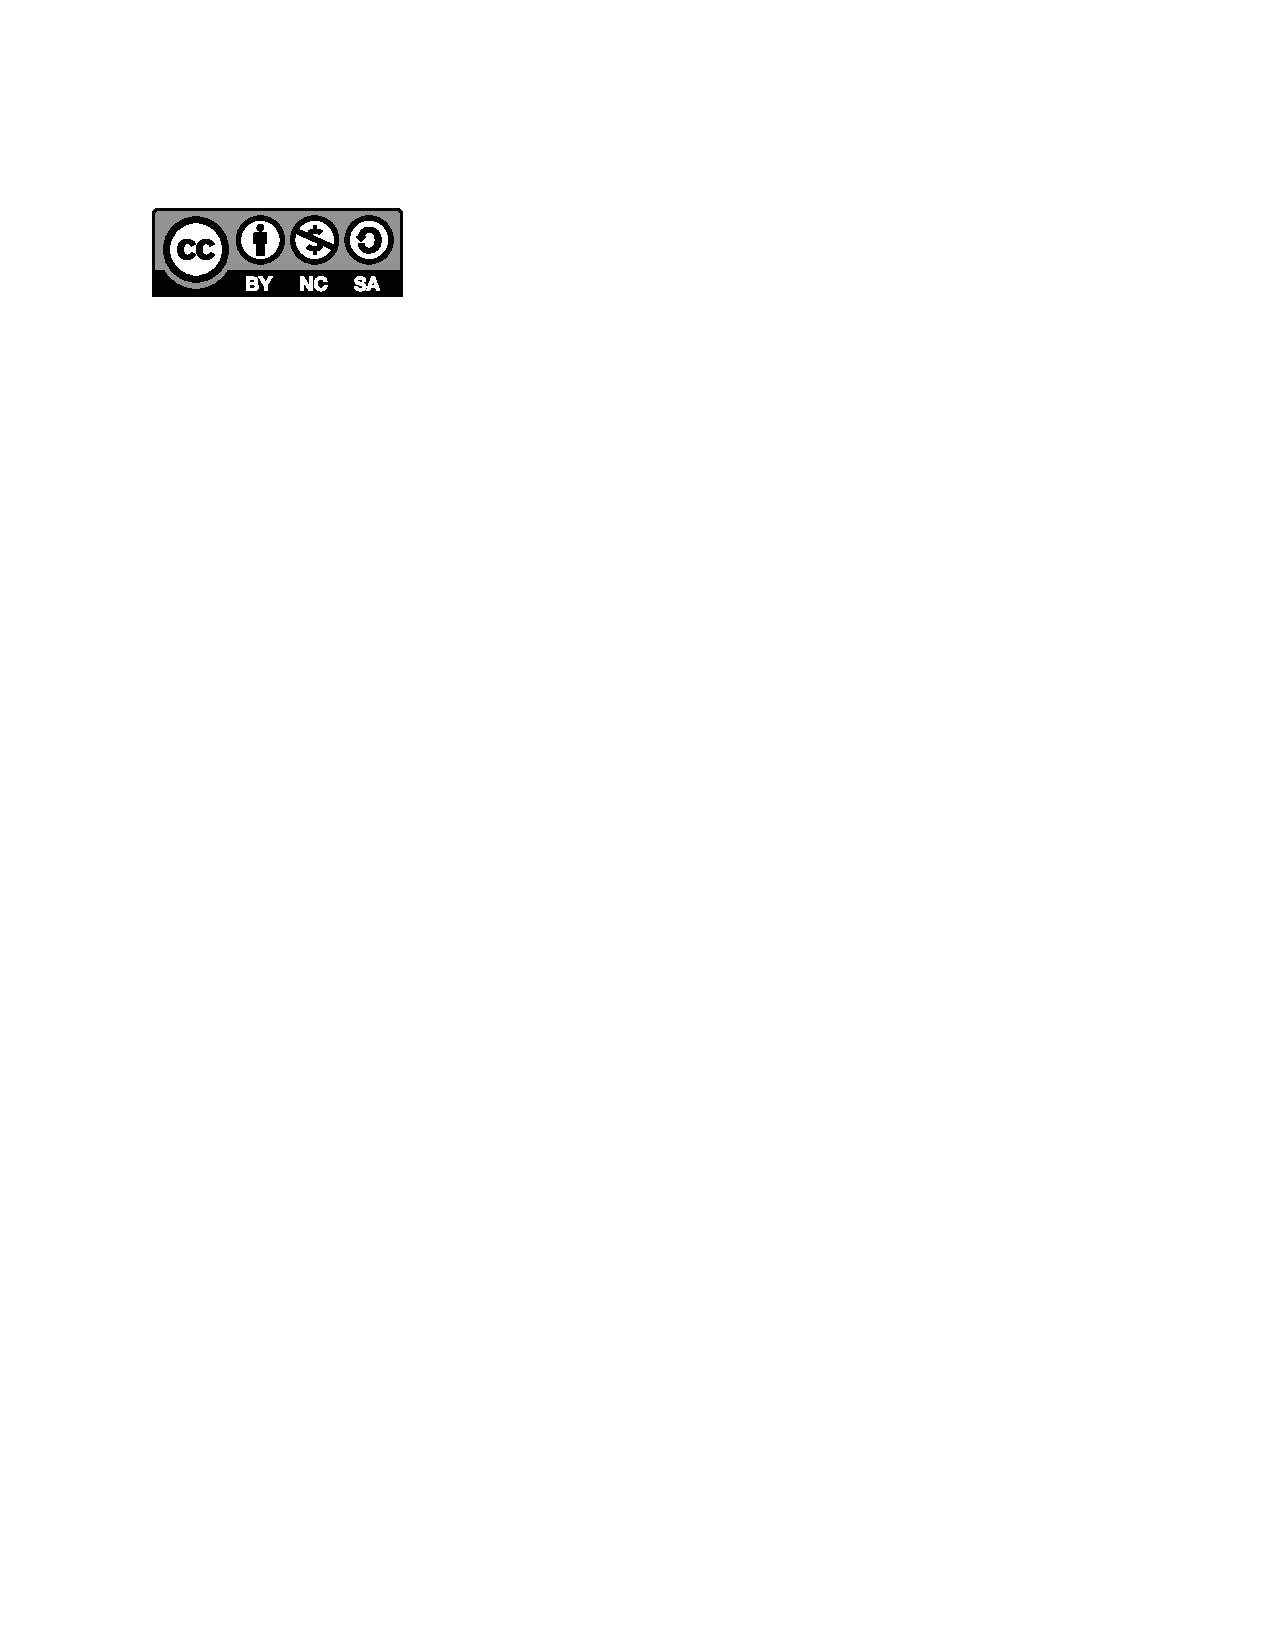
\includegraphics{CR_Logo.pdf}
\end{wrapfigure}
Unless otherwise noted, this textbook is licensed with a Creative
Commons\\
Attribution NonCommercial-ShareAlike 4.0 license:\\
\url{https://creativecommons.org/licenses/by-nc-sa/4.0}. You are free \text{to copy,}\break share, adapt, remix, transform, and build upon
the material for any not primarily commercial
purpose, as long as you follow the terms of the license:\\
\url{https://creativecommons.org/licenses/by-nc-sa/4.0/legalcode}.

This work is published by the Kevin T. Crofton Department of Aerospace and Ocean Engineering in association
with Virginia Tech Publishing, a division of the University Libraries at Virginia Tech.

Virginia Tech Publishing. 560 Drillfield Drive, Blacksburg, VA 24061,
USA. \url{publishing@vt.edu}.

Kevin T. Crofton Department of Aerospace and Ocean Engineering.
Randolph Hall, RM 215, Virginia Tech\\
460 Old Turner Street, Blacksburg, VA 24061, USA .

Suggested citation: Johnson, Eric R. (2021) {Aerospace
Structures}. Blacksburg: Virginia Tech Kevin T. Crofton\\
Department of Aerospace and Ocean Engineering. \url{https://doi.org/10.21061/AerospaceStructures}.
Licensed with CC BY NC-SA 4.0.
\url{https://creatvecommons.org/licenses/by-nc-sa/4.0}

Peer Review: This book has undergone single-blind peer review by seven external subject matter experts.

Publication of this book was made possible in part through funding
from VIVA (the Virtual Library of Virginia),\\
the Open Education Initiative at the University Libraries
at Virginia Tech, and Virginia Tech Publishing.

Accessibility Statement: Virginia Tech Publishing is committed to
making its publications accessible in\\
accordance with the Americans with Disabilities Act of 1990. The ePub
version of this book is accessible. The\\
\LaTeX\ source files also include alternative text for all images and figures.

Publication Cataloging Information\\
Johnson, Eric R., author\\
\hspace*{1em}Aerospace Structures\,/\,Eric R. Johnson\\
\hspace*{1em}Pages cm\\
\hspace*{1em}ISBN 978-1-949373-44-8 (print)\\
\hspace*{1em}ISBN 978-1-949373-46-2 (PDF)\\
\hspace*{1em}ISBN 978-1-949373-45-5 (LaTeX)\\
\hspace*{1em}ISBN 978-1-949373-65-3 (ePub)\\
\hspace*{1em}DOI: \url{https://doi.org/10.21061/Aerospace Structures}\\
\hspace*{2em}Airframes---Mathematical models.\\
\hspace*{2em}Failure analysis (Engineering)---Mathematical models.\\
\hspace*{2em}Structural analysis (Engineering)---Mathematical
models.\\
1.\hspace{24pt}Title\\
\phantom{1.}\hspace{24pt}TL671.6.J64 2022\\
\phantom{1.}\hspace{24pt}629.134\\
Cover Design (licensed CC BY 4.0): Kindred Grey\\
Cover image: Adapted from (c) Tom Cleary. Unsplash license
\url{https://unsplash.com/license}. Retrieved from\\
\url{https://unsplash.com/photos/MFZYwRJnKAo}.

\enlargethispage{2\baselineskip}

\textbf{About the author}\\
{\raggedright Eric Raymond Johnson is emeritus professor of aerospace and ocean engineering at Virginia Tech. He earned his doctoral degree in applied mechanics from the University of Michigan in 1976, and from 1976 to 2003 was a member of the engineering faculty at Virginia Tech. Dr. Johnson s research area is composite structures. Research activities include the mechanics of the response and failure of advanced composite material structures with applications to flight and land vehicles, buckling and post-buckling of plates and shells, progressive failure analysis for the prediction of energy absorption in laminated composites and in bonded joints, and fracture mechanics. He has sixty-four publications in structural mechanics, and has been awarded research funding from government agencies and industries. He is a senior member of the American Institute of Aeronautics and Astro-nautics and a member of the American Society of Mechanical Engineers.\par}
\end{copyrt}

\thispagestyle{empty}

\clearpage

\null\vspace{-2.5\baselineskip}\vspace{-50pt}%

\noindent{\fontsize{18}{22}\fontseries{b}\selectfont{Features of This Open
Textbook}}

\vspace{6pt}

{\parindent=0pt\setlength\parskip{9pt}

{\small
\textbf{Additional Resources}\\
The following resources are freely available at
\url{http://hdl.handle.net/10919/102306}.\\
\begin{tabular}[t]{@{}l@{\hskip46pt}l@{}}
Downloadable PDF & Errata and error reporting form\\
Print edition ordering details& Links to collaborator portal and listserv
\end{tabular}\\
LaTeX source files\par}

If you are an instructor reviewing, adopting, or adapting this
textbook, please help us understand your use by\\
completing this form:
\url{http://bit.ly/interest-aerospace-structures}

\vspace{6pt}

{\setlength{\columnsep}{9pt}

\begin{wrapfigure}[6]{l}{122pt}
\vspace{-18pt}
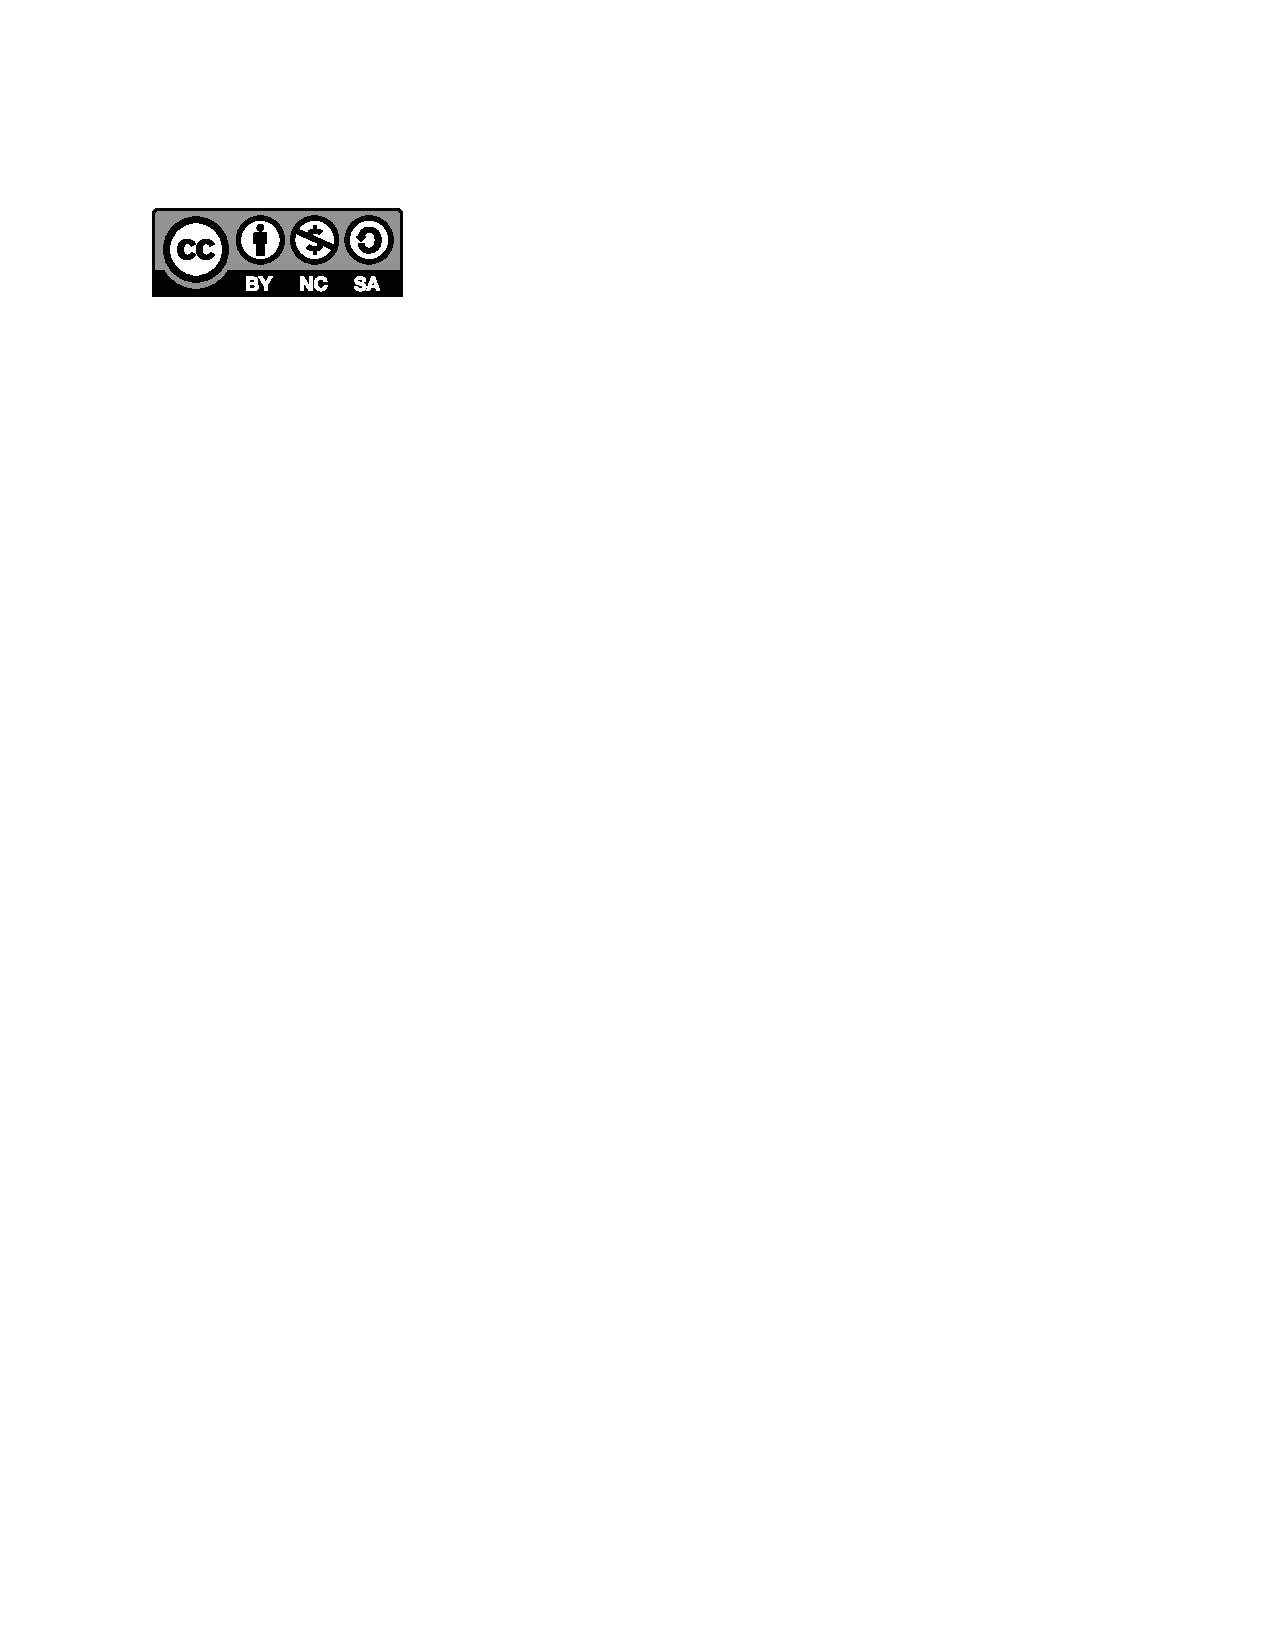
\includegraphics{CR_Logo.pdf}
\end{wrapfigure}
You are free to copy, share, adapt, remix, transform, and build upon
the material\\
for any not primarily commercial purpose, as long as you follow the
terms of the\\
license: \url{https://creativecommons.org/licenses/by-nc-sa/4.0}.

}

\vspace{18pt}

\begin{framed}
\begin{tabular}[t]{@{}ll@{}}
You must&\\[3pt]
\smash{\raisebox{-29pt}{
\includegraphics[width=38pt,height=38pt]{by.eps}}}
&Attribute---You must give appropriate credit, provide a link to the
license, and indicate if changes\\
&were made. You may do so in any reasonable matter, but not in any
way that the licensor endorse\\
&you or your use.\\[6pt]
&\footnotesize Suggested citation for an adapted work:
Adapted by \_\_\_[your name]\_\_\_from \textcopyright\ Eric R Johnson,  Aerospace Structures,\\
&\footnotesize\url{https://doi.org/10.21061/Aerospace Structures}, CC B NC SA 4.0, \url{https://creativecommons.org/licenses/by-nc-sa/4.0}
\end{tabular}
\end{framed}

\vspace{6pt}

\begin{framed}
\begin{tabular}[t]{@{}lp{30pc}@{}}
You must&\\[3pt]
\smash{\raisebox{-32pt}{
\includegraphics{CR_Logo_2.pdf}}} &ShareAlike---If you remix, transform, or build on the material, you must distribute your contributions
under the same license as the original.\\\\
\end{tabular}
\end{framed}

\vspace{6pt}

\begin{framed}
\begin{tabular}[t]{@{}lp{30pc}@{}}
You may not: &\\[3pt]
\smash{\raisebox{-32pt}{
\includegraphics[width=38pt,height=38pt]{nc.eps}}}
 &Noncommercial---You may not use the material for uses that are primarily intended for or directed
toward commercial advantage or monetary compensation\\\\
\end{tabular}
\end{framed}

%\enlargethispage{3\baselineskip}
\thispagestyle{empty}

You may not:\\
Add any additional restrictions---You may not apply legal terms or
technological measures that legally restrict\\
others from doing anything the license permits.

\vspace{6pt}

\begin{framed}
If adopting or building upon, you are encouraged to:\\[5pt]
$\smallbullet${\quad}Register your use at
\url{http://bit.ly/interest-aerospace-structures}\\[5pt]
$\smallbullet${\quad}Incorporate only your own original work or works with a
CC BY, CC BY NC, or CC BY NC SA license.\\[5pt]
$\smallbullet${\quad}Attribute all added content.\\[5pt]
$\smallbullet${\quad}Have your work peer reviewed.\\[5pt]
$\smallbullet${\quad}Include a transformation statement that describes changes, additions, accessibility features, and any subsequent
peer review.\\[5pt]
$\smallbullet${\quad}If incorporating text or figures under an informed fair
use analysis, mark them as such and cite them.\\[5pt]
$\smallbullet${\quad}Share your contributions in the collaborator portal or
on the listserv.

\vspace{6pt}

\hbox{\begin{minipage}[t]{16pc}
\textbf{Suggestions for creating and adapting}\\
Create and share learning tools and study aids.\\
Translate. Modify the sequence or structure.\\
%\hspace*{1em}\href{libretext.org}{libretext.org}\\
Add or modify problems and examples.\\
Transform or build upon in other formats.
\end{minipage}\ignorespaces\hspace{3pc}\ignorespaces%
\begin{minipage}[t]{15pc}
\textbf{Adaptation resources}\\
LaTeX source files are available or\\
Adapt on your own at \url{https://libretext.org}
\end{minipage}}
\vspace{-2pt}
\end{framed}

\vspace{-6pt}

{\leftskip=10.5pt
\noindent\textbf{Submit suggestions and comments}\\
Submit suggestions (anonymous):
\url{http://bit.ly/feedback-aerospace-structures}\\
\href{mailto:publishing@vt.edu}{Email: publishing@vt.edu}\par
}

\par}

\thispagestyle{empty}
\clearpage

\clearemptydoublepage

%\tableofcontents
\pagestyle{fmheadings}
\makeatletter
\@makestocchapterhead{Table of Contents}%
\thispagestyle{fmplain}%

{\setlength\parskip{0pt}

%\clearpage
%\null\vspace{-2.5\baselineskip}\vspace{-30pt}%%

%\clearpage
%\null\vspace{-2.5\baselineskip}\vspace{-41pt}\vspace{-15pt}%

\contentsline {chapter}{\numberline {1}Function of flight vehicle structural members}{1}{chapter.1}\protected@file@percent 
\contentsline {section}{\numberline {1.1}Space truss/frame}{1}{section.1.1}\protected@file@percent 
\contentsline {section}{\numberline {1.2}Monocoque and semimonocoque constructions}{2}{section.1.2}\protected@file@percent 
\contentsline {section}{\numberline {1.3}Rocket structure}{3}{section.1.3}\protected@file@percent 
\contentsline {section}{\numberline {1.4}References}{5}{section.1.4}\protected@file@percent 

\contentsline {chapter}{\numberline {2}Aircraft loads}{7}{chapter.2}\protected@file@percent 
\contentsline {section}{\numberline {2.1}Aircraft design process}{7}{section.2.1}\protected@file@percent 
\contentsline {section}{\numberline {2.2}Inertia loads}{7}{section.2.2}\protected@file@percent 
\contentsline {subsection}{\numberline {2.2.1}Coordinate systems and Newton's laws of motion}{8}{subsection.2.2.1}\protected@file@percent 
\contentsline {subsection}{\numberline {2.2.2}Principle of D'Alembert}{9}{subsection.2.2.2}\protected@file@percent 
\contentsline {subsection}{\numberline {2.2.3}Relative velocity and acceleration}{10}{subsection.2.2.3}\protected@file@percent 
\contentsline {subsection}{\numberline {2.2.4}Uniform linear and angular accelerations}{11}{subsection.2.2.4}\protected@file@percent 
\contentsline {section}{\numberline {2.3}Load factors}{11}{section.2.3}\protected@file@percent 
\contentsline {section}{\numberline {2.4}The V-n diagram}{13}{section.2.4}\protected@file@percent 
\contentsline {subsection}{\numberline {2.4.1}Airplane design requirements}{13}{subsection.2.4.1}\protected@file@percent 
\contentsline {subsection}{\numberline {2.4.2}Regulations}{13}{subsection.2.4.2}\protected@file@percent 
\contentsline {subsection}{\numberline {2.4.3}Specified data}{13}{subsection.2.4.3}\protected@file@percent 
\contentsline {subsection}{\numberline {2.4.4}Basic maneuver V-n diagram}{14}{subsection.2.4.4}\protected@file@percent 
\contentsline {subsection}{\numberline {2.4.5}Aerodynamic data}{14}{subsection.2.4.5}\protected@file@percent 
\contentsline {paragraph}{Methods of data acquisition.}{15}{section*.1}\protected@file@percent 
\contentsline {subsection}{\numberline {2.4.6}Maneuver V-n diagram including aerodynamic stall}{18}{subsection.2.4.6}\protected@file@percent 
\contentsline {paragraph}{Transport category airplanes.}{19}{section*.2}\protected@file@percent 
\contentsline {section}{\numberline {2.5}Design gust load factors}{19}{section.2.5}\protected@file@percent 
\contentsline {subsection}{\numberline {2.5.1}Gust alleviation factor}{20}{subsection.2.5.1}\protected@file@percent 
\contentsline {subsection}{\numberline {2.5.2}Gust load factor}{21}{subsection.2.5.2}\protected@file@percent 
\contentsline {subsection}{\numberline {2.5.3}NACA discrete gust conditions}{21}{subsection.2.5.3}\protected@file@percent 
\contentsline {subsection}{\numberline {2.5.4}Design V-n diagram}{21}{subsection.2.5.4}\protected@file@percent 
\contentsline {section}{\numberline {2.6}Design V-n diagram example}{21}{section.2.6}\protected@file@percent 
\contentsline {paragraph}{Problem statement:}{23}{section*.3}\protected@file@percent 
\contentsline {section}{\numberline {2.7}References}{25}{section.2.7}\protected@file@percent 
\contentsline {section}{\numberline {2.8}Practice exercises}{25}{section.2.8}\protected@file@percent 

\contentsline {chapter}{\numberline {3}Elements of a thin-walled bar\nobreakspace  {}theory}{29}{chapter.3}\protected@file@percent 
\contentsline {section}{\numberline {3.1}Open cross section}{29}{section.3.1}\protected@file@percent 
%\contentsline {subsubsection}{Centroid C.}{31}{section*.1}\protected@file@percent 
%\contentsline {subsubsection}{Shear center S.C.}{32}{section*.2}\protected@file@percent 
\contentsline {section}{\numberline {3.2}Contour geometry}{31}{section.3.2}\protected@file@percent 
\contentsline {section}{\numberline {3.3}Displacements}{33}{section.3.3}\protected@file@percent 
\contentsline {section}{\numberline {3.4}Strains}{35}{section.3.4}\protected@file@percent 
\contentsline {section}{\numberline {3.5}Stresses, stress resultants and bar resultants}{36}{section.3.5}\protected@file@percent 
\contentsline {section}{\numberline {3.6}External loads and equilibrium of an element of the bar}{38}{section.3.6}\protected@file@percent 
\contentsline {subsection}{\numberline {3.6.1}Differential equilibrium equations}{39}{subsection.3.6.1}\protected@file@percent 
%\contentsline {subsubsection}{Axial equilibrium.}{41}{section*.3}\protected@file@percent 
%\contentsline {subsubsection}{Bending in the \textit  {y-z} plane.}{42}{section*.4}\protected@file@percent 
%\contentsline {subsubsection}{Bending in the \textit  {x-z} plane.}{42}{section*.5}\protected@file@percent 
%\contentsline {subsubsection}{Torsion.}{42}{section*.6}\protected@file@percent 
\contentsline {section}{\numberline {3.7}Hooke's law}{41}{section.3.7}\protected@file@percent 
\contentsline {subsection}{\numberline {3.7.1}Effect of thermal expansion}{41}{subsection.3.7.1}\protected@file@percent 
\contentsline {subsection}{\numberline {3.7.2}Material law for extension and bending}{42}{subsection.3.7.2}\protected@file@percent 
%\contentsline {subsubsection}{{Locating the origin of the cross-sectional Cartesian system at the centroid decouples the extensional and bending responses in the material law (\ref  {eq3.79}) for the bar.}}{45}{section*.7}\protected@file@percent 
\contentsline {section}{\numberline {3.8}Shear flow due to the transverse shear forces}{45}{section.3.8}\protected@file@percent 
\contentsline {subsection}{\numberline {3.8.1} Open cross-sectional contour}{47}{subsection.3.8.1}\protected@file@percent 

\clearpage
\null\vspace{-2.5\baselineskip}\vspace{-30pt}%

\contentsline {subsection}{\numberline {3.8.2}Location of the shear center for an open cross section}{49}{subsection.3.8.2}\protected@file@percent 
\contentsline {subsection}{\numberline {3.8.3}Notes concerning the shear center}{53}{subsection.3.8.3}\protected@file@percent 
\contentsline {section}{\numberline {3.9}Torsion of an open section with a straight contour}{53}{section.3.9}\protected@file@percent 
%\contentsline {subsubsection}{Displacements and strains.}{56}{section*.24}\protected@file@percent 
%\contentsline {subsubsection}{Stress resultants and equilibrium.}{56}{section*.25}\protected@file@percent 
%\contentsline {subsubsection}{Governing boundary value problem.}{57}{section*.26}\protected@file@percent 
%\contentsline {subsubsection}{Warping of the cross section.}{59}{section*.27}\protected@file@percent 
\contentsline {subsection}{\numberline {3.9.1}Torsion of built-up open sections}{58}{subsection.3.9.1}\protected@file@percent 
\contentsline {section}{\numberline {3.10}Inclusion of stringers in the analysis of the cross section}{60}{section.3.10}\protected@file@percent 
\contentsline {subsection}{\numberline {3.10.1}Effect of stringers on the shear flow distribution}{60}{subsection.3.10.1}\protected@file@percent 
\contentsline {section}{\numberline {3.11}Closed cross-sectional contour}{62}{section.3.11}\protected@file@percent 
\contentsline {subsection}{\numberline {3.11.1}Twist per unit longitudinal length}{63}{subsection.3.11.1}\protected@file@percent 
\contentsline {subsection}{\numberline {3.11.2}Location of the shear center and the final expression for the\break shear flow}{64}{subsection.3.11.2}\protected@file@percent 
%\contentsline {subsubsection}{Solution to part (a).}{68}{section*.28}\protected@file@percent 
%\contentsline {subsubsection}{Solution to part (b).}{69}{section*.29}\protected@file@percent 
%\contentsline {subsubsection}{Solution to part c.}{71}{section*.32}\protected@file@percent 
\contentsline {section}{\numberline {3.12}References}{69}{section.3.12}\protected@file@percent 

\contentsline {chapter}{\numberline {4}Some aspects of the structural analysis}{71}{chapter.4}\protected@file@percent 
\contentsline {section}{\numberline {4.1}Review of the thin-wall bar theory}{72}{section.4.1}\protected@file@percent 
\contentsline {subsection}{\numberline {4.1.1}Extension and bending}{72}{subsection.4.1.1}\protected@file@percent 
\contentsline {subsection}{\numberline {4.1.2}Shear stresses in open and closed sections}{73}{subsection.4.1.2}\protected@file@percent 
\contentsline {subsection}{\numberline {4.1.3}Hooke's law for transverse shear and torsion}{76}{subsection.4.1.3}\protected@file@percent 
\contentsline {section}{\numberline {4.2}Yield criteria}{77}{section.4.2}\protected@file@percent 
\contentsline {section}{\numberline {4.3}Structural analyses for extension and flexure}{78}{section.4.3}\protected@file@percent 
\contentsline {subsection}{\numberline {4.3.1}Bending moment diagrams}{78}{subsection.4.3.1}\protected@file@percent 
\contentsline {subsection}{\numberline {4.3.2}Buoyancy force distribution on ships}{82}{subsection.4.3.2}\protected@file@percent 
\contentsline {subsection}{\numberline {4.3.3}Properties of plane areas}{84}{subsection.4.3.3}\protected@file@percent 
%\contentsline {subsubsection}{Parallel axis theorem.}{86}{section*.3}\protected@file@percent 
%\contentsline {subsubsection}{Radii of gyration.}{87}{section*.4}\protected@file@percent 
%\contentsline {subsubsection}{Composite area technique.}{88}{section*.5}\protected@file@percent 
\contentsline {subsection}{\numberline {4.3.4}Neutral axis of the cross section}{88}{subsection.4.3.4}\protected@file@percent 
\contentsline {section}{\numberline {4.4}Structural analyses for transverse shear and torsion}{95}{section.4.4}\protected@file@percent 
%\contentsline {subsubsection}{Solution to part (a).}{98}{section*.6}\protected@file@percent 
%\contentsline {subsubsection}{Solution to part (b).}{99}{section*.7}\protected@file@percent 
%\contentsline {subsubsection}{Solution to part (c).}{99}{section*.8}\protected@file@percent 
%\contentsline {subsubsection}{Solution to part (d).}{100}{section*.9}\protected@file@percent 
%\contentsline {subsubsection}{Solution to part (a).}{101}{section*.10}\protected@file@percent 
%\contentsline {subsubsection}{Solution part to (b).}{101}{section*.11}\protected@file@percent 
%\contentsline {subsubsection}{Solution to part (c).}{102}{section*.12}\protected@file@percent 
%\contentsline {subsubsection}{Solution to part (d).}{103}{section*.13}\protected@file@percent 
%\contentsline {subsubsection}{Solution to part (e).}{103}{section*.14}\protected@file@percent 
\contentsline {subsection}{\numberline {4.4.1}Resultant of uniform shear flow}{102}{subsection.4.4.1}\protected@file@percent 
\contentsline {subsection}{\numberline {4.4.2}Torsion of a hybrid section}{104}{subsection.4.4.2}\protected@file@percent 
\contentsline {section}{\numberline {4.5}References}{116}{section.4.5}\protected@file@percent 
\contentsline {section}{\numberline {4.6}Practice exercises}{116}{section.4.6}\protected@file@percent 

\contentsline {chapter}{\numberline {5}Work and energy methods}{121}{chapter.5}\protected@file@percent 
\contentsline {section}{\numberline {5.1}Hooke's law and its corollaries}{121}{section.5.1}\protected@file@percent 
\contentsline {subsection}{\numberline {5.1.1}Work of the external loads}{122}{subsection.5.1.1}\protected@file@percent 
\contentsline {subsection}{\numberline {5.1.2}Maxwell's reciprocal theorem}{123}{subsection.5.1.2}\protected@file@percent 
\contentsline {section}{\numberline {5.2}Extensions of Hooke's law to include a couple and rotation}{124}{section.5.2}\protected@file@percent 
\contentsline {subsection}{\numberline {5.2.1}Generalized forces and displacements}{125}{subsection.5.2.1}\protected@file@percent 
\contentsline {subsection}{\numberline {5.2.2}Stiffness influence coefficients}{125}{subsection.5.2.2}\protected@file@percent 
\contentsline {section}{\numberline {5.3}Strain energy density functions}{127}{section.5.3}\protected@file@percent 
\contentsline {subsection}{\numberline {5.3.1}Strain energy density in uniaxial normal strain}{127}{subsection.5.3.1}\protected@file@percent 
\contentsline {subsection}{\numberline {5.3.2}Complementary energy density in uniaxial normal stress}{129}{subsection.5.3.2}\protected@file@percent 
\contentsline {subsection}{\numberline {5.3.3}Strain energy density in shear}{130}{subsection.5.3.3}\protected@file@percent 
\contentsline {section}{\numberline {5.4}Strain energy for extension and bending of a thin-walled bar}{131}{section.5.4}\protected@file@percent 
\contentsline {section}{\numberline {5.5}Strain energy for shear and torsion of a thin-walled bar}{132}{section.5.5}\protected@file@percent 
\contentsline {subsection}{\numberline {5.5.1}Open cross-sectional contour}{132}{subsection.5.5.1}\protected@file@percent 
\contentsline {subsection}{\numberline {5.5.2}Closed cross-sectional contour}{133}{subsection.5.5.2}\protected@file@percent 
\contentsline {subsection}{\numberline {5.5.3}Material law for transverse shear and torsion}{134}{subsection.5.5.3}\protected@file@percent 
\contentsline {section}{\numberline {5.6}Total strain energy expressions for a thin-walled bar}{135}{section.5.6}\protected@file@percent 
\contentsline {section}{\numberline {5.7} Castigliano's first theorem}{136}{section.5.7}\protected@file@percent 
\contentsline {section}{\numberline {5.8}Castigliano's second theorem}{139}{section.5.8}\protected@file@percent 
\contentsline {section}{\numberline {5.9}References}{141}{section.5.9}\protected@file@percent 


\clearpage
\null\vspace{-2.5\baselineskip}\vspace{-41pt}\vspace{-15pt}%

\contentsline {chapter}{\numberline {6}Applications of Castigliano's Theorems}{143}{chapter.6}\protected@file@percent 
\contentsline {section}{\numberline {6.1}Coplanar trusses}{143}{section.6.1}\protected@file@percent 
\contentsline {subsection}{\numberline {6.1.1}Castigliano’s first theorem}{143}{subsection.6.1.1}\protected@file@percent 
%\contentsline {subsubsection}{Solution.}{4}{section*.1}\protected@file@percent 
%\contentsline {subsubsection}{Solution.}{5}{section*.10}\protected@file@percent 
\contentsline {subsection}{\numberline {6.1.2}Castigliano's second theorem for a statically determinate truss}{148}{subsection.6.1.2}\protected@file@percent 
%\contentsline {subsubsection}{A note on static determinacy:}{6}{section*.20}\protected@file@percent 
%\contentsline {subsubsection}{Solution.}{6}{section*.21}\protected@file@percent 
\contentsline {section}{\numberline {6.2}Beam structures}{150}{section.6.2}\protected@file@percent 
%\contentsline {subsubsection}{Solution.}{8}{section*.30}\protected@file@percent 
\contentsline {subsection}{\numberline {6.2.1}Castigliano's second theorem}{151}{subsection.6.2.1}\protected@file@percent 
%\contentsline {subsubsection}{Solution.}{10}{section*.46}\protected@file@percent 
%\contentsline {subsubsection}{Solution to part (a).}{13}{section*.71}\protected@file@percent 
%\contentsline {subsubsection}{Solution to part (b).}{14}{section*.79}\protected@file@percent 
%\contentsline {subsubsection}{Solution to part (c).}{15}{section*.89}\protected@file@percent 
\contentsline {section}{\numberline {6.3}Coplanar frames}{159}{section.6.3}\protected@file@percent 
%\contentsline {subsubsection}{Solution.}{17}{section*.98}\protected@file@percent 
\contentsline {section}{\numberline {6.4}Castigliano's second theorem and statically indeterminate structures}{161}{section.6.4}\protected@file@percent 
%\contentsline {subsubsection}{Solution.}{20}{section*.124}\protected@file@percent 
%\contentsline {subsubsection}{Solution.}{23}{section*.125}\protected@file@percent 
\contentsline {subsection}{\numberline {6.4.1}Function of a Turnbuckle}{166}{subsection.6.4.1}\protected@file@percent 
%\contentsline {subsubsection}{Solution.}{25}{section*.126}\protected@file@percent 
\contentsline {section}{\numberline {6.5}References}{169}{section.6.5}\protected@file@percent 
\contentsline {section}{\numberline {6.6}Practice exercises}{169}{section.6.6}\protected@file@percent 

\contentsline {chapter}{\numberline {7}Arches, rings and fuselage frames}{175}{chapter.7}\protected@file@percent 
\contentsline {section}{\numberline {7.1}Coplanar curved bars}{175}{section.7.1}\protected@file@percent 
\contentsline {subsection}{\numberline {7.1.1}Displacements and strain}{176}{subsection.7.1.1}\protected@file@percent 
\contentsline {subsection}{\numberline {7.1.2}Normal stress, stress resultants, and strain energy}{178}{subsection.7.1.2}\protected@file@percent 
%\contentsline {subsubsection}{Solution.}{8}{section*.5}\protected@file@percent 
\contentsline {section}{\numberline {7.2}Strain-displacement and Hooke's law for thin curved bars}{184}{section.7.2}\protected@file@percent 
%\contentsline {subsubsection}{Solution to part (a).}{10}{section*.18}\protected@file@percent 
%\contentsline {subsubsection}{Solution to part (b).}{12}{section*.27}\protected@file@percent 
%\contentsline {subsubsection}{Solution.}{12}{section*.30}\protected@file@percent 
\contentsline {section}{\numberline {7.3}Differential equilibrium equations of a curved bar}{189}{section.7.3}\protected@file@percent 
\contentsline {section}{\numberline {7.4}Loads on fuselage frames}{192}{section.7.4}\protected@file@percent 
%\contentsline {subsubsection}{Solution.}{20}{section*.49}\protected@file@percent 
%\contentsline {subsubsection}{Solution to part 1.}{23}{section*.79}\protected@file@percent 
%\contentsline {subsubsection}{Solution to part 2.}{24}{section*.85}\protected@file@percent 
%\contentsline {subsubsection}{Solution to part 3.}{25}{section*.94}\protected@file@percent 
%\contentsline {subsubsection}{Solution to part 4.}{25}{section*.99}\protected@file@percent 
%\contentsline {subsubsection}{Solution to part 5.}{25}{section*.101}\protected@file@percent 
%\contentsline {subsubsection}{Solution to part 6.}{26}{section*.114}\protected@file@percent 
\contentsline {section}{\numberline {7.5}References}{202}{section.7.5}\protected@file@percent 
\contentsline {section}{\numberline {7.6}Practice exercises}{203}{section.7.6}\protected@file@percent 
%\contentsline {subsubsection}{Hint.}{30}{section*.125}\protected@file@percent 

\contentsline {chapter}{\numberline {8}Laminated bars of fiber-reinforced polymer composites}{205}{chapter.8}\protected@file@percent 
\contentsline {section}{\numberline {8.1}Fibrous composites}{205}{section.8.1}\protected@file@percent 
\contentsline {subsection}{\numberline {8.1.1}Material law in principal directions}{206}{subsection.8.1.1}\protected@file@percent 
\contentsline {subsection}{\numberline {8.1.2}Compliance matrix in bar coordinate directions}{207}{subsection.8.1.2}\protected@file@percent 
\contentsline {subsection}{\numberline {8.1.3}Plane stress}{210}{subsection.8.1.3}\protected@file@percent 
\contentsline {subsection}{\numberline {8.1.4}Nomenclature of composite materials}{212}{subsection.8.1.4}\protected@file@percent 
%\contentsline {subsubsection}{Solution.}{8}{section*.1}\protected@file@percent 
\contentsline {subsection}{\numberline {8.1.5}Laminated wall}{213}{subsection.8.1.5}\protected@file@percent 
%\contentsline {subsubsection}{Solution to part (a).}{10}{section*.8}\protected@file@percent 
%\contentsline {subsubsection}{Solution to part (b).}{10}{section*.9}\protected@file@percent 
\contentsline {subsection}{\numberline {8.1.6}Balanced and specially orthotropic laminates}{215}{subsection.8.1.6}\protected@file@percent 
\contentsline {section}{\numberline {8.2}Composite thin-walled bar with a closed cross-sectional contour}{215}{section.8.2}\protected@file@percent 
\contentsline {subsection}{\numberline {8.2.1}Anisotropic Hooke's law for the cross section}{217}{subsection.8.2.1}\protected@file@percent 
\contentsline {subsection}{\numberline {8.2.2}Expressions for the shear flow and normal stress resultant}{218}{subsection.8.2.2}\protected@file@percent 
\contentsline {subsection}{\numberline {8.2.3}Complementary work and energy}{220}{subsection.8.2.3}\protected@file@percent 
\contentsline {subsection}{\numberline {8.2.4}Cross-sectional compliance matrix}{223}{subsection.8.2.4}\protected@file@percent 
%\contentsline {subsubsection}{Solution.}{20}{section*.10}\protected@file@percent 
%\contentsline {subsubsection}{Solution.}{22}{section*.27}\protected@file@percent 
\contentsline {section}{\numberline {8.3}Open cross-sectional contour}{229}{section.8.3}\protected@file@percent 
\contentsline {section}{\numberline {8.4}Uniform torsion of an FRP bar with a rectangular cross section}{230}{section.8.4}\protected@file@percent 
\contentsline {subsection}{\numberline {8.4.1}Displacements}{231}{subsection.8.4.1}\protected@file@percent 
\contentsline {subsection}{\numberline {8.4.2}Equilibrium}{234}{subsection.8.4.2}\protected@file@percent 
\contentsline {subsection}{\numberline {8.4.3}Static equivalence}{235}{subsection.8.4.3}\protected@file@percent 
\contentsline {subsection}{\numberline {8.4.4}Principle of complementary virtual work}{237}{subsection.8.4.4}\protected@file@percent 
%\contentsline {subsubsection}{Solution to part (a).}{37}{section*.38}\protected@file@percent 
%\contentsline {subsubsection}{Solution to part (b).}{38}{section*.51}\protected@file@percent 
\contentsline {section}{\numberline {8.5}References}{245}{section.8.5}\protected@file@percent 


\contentsline {chapter}{\numberline {9}Failure initiation in FRP composites}{247}{chapter.9}\protected@file@percent 
\contentsline {section}{\numberline {9.1}Strength of a composite ply}{247}{section.9.1}\protected@file@percent 
\contentsline {subsection}{\numberline {9.1.1}Puck's failure criterion}{248}{subsection.9.1.1}\protected@file@percent 
%\contentsline {subsubsection}{Matrix mode A.}{3}{section*.1}\protected@file@percent 
%\contentsline {subsubsection}{Matrix modes B and C.}{5}{section*.2}\protected@file@percent 
%\contentsline {subsubsection}{Fiber modes.}{8}{section*.3}\protected@file@percent 
\contentsline {subsection}{\numberline {9.1.2}Matrix failure criteria for a plane stress state}{254}{subsection.9.1.2}\protected@file@percent 
%\contentsline {subsubsection}{Modes B and C for a plane stress state.}{9}{section*.4}\protected@file@percent 
%\contentsline {subsubsection}{Transverse shear strength.}{10}{section*.5}\protected@file@percent 

\clearpage
\null\vspace{-2.5\baselineskip}\vspace{-30pt}%

\contentsline {section}{\numberline {9.2}Stresses in the principal material directions}{258}{section.9.2}\protected@file@percent 
%\contentsline {subsubsection}{Computations for $\beta =30^{\circ }$.}{14}{section*.13}\protected@file@percent 
%\contentsline {subsubsection}{Computations for $\beta =150^{\circ }$.}{14}{section*.17}\protected@file@percent 
\contentsline {section}{\numberline {9.3}References}{263}{section.9.3}\protected@file@percent 

\contentsline {chapter}{\numberline {10}Structural stability of discrete conservative systems}{265}{chapter.10}\protected@file@percent 
\contentsline {section}{\numberline {10.1}Model A: stable symmetric bifurcation buckling}{265}{section.10.1}\protected@file@percent 
\contentsline {subsection}{\numberline {10.1.1}Equilibrium method}{266}{subsection.10.1.1}\protected@file@percent 
%\contentsline {subsubsection}{Small $\boldsymbol  {\theta }$ analysis.}{3}{section*.1}\protected@file@percent 
\contentsline {subsection}{\numberline {10.1.2}Kinetic method}{267}{subsection.10.1.2}\protected@file@percent 
\contentsline {subsection}{\numberline {10.1.3}Energy method}{269}{subsection.10.1.3}\protected@file@percent 
%\contentsline {subsubsection}{Theorem.}{5}{section*.2}\protected@file@percent 
\contentsline {subsection}{\numberline {10.1.4}Eccentric load}{271}{subsection.10.1.4}\protected@file@percent 
\contentsline {subsection}{\numberline {10.1.5}Initial angle}{272}{subsection.10.1.5}\protected@file@percent 
%\contentsline {subsubsection}{Discussion.}{9}{section*.3}\protected@file@percent 
\contentsline {section}{\numberline {10.2}Model B: unstable symmetric bifurcation}{273}{section.10.2}\protected@file@percent 
\contentsline {subsection}{\numberline {10.2.1}Initial angle imperfection}{275}{subsection.10.2.1}\protected@file@percent 
%\contentsline {subsubsection}{Discussion.}{12}{section*.4}\protected@file@percent 
\contentsline {section}{\numberline {10.3}Model C: asymmetric bifurcation}{277}{section.10.3}\protected@file@percent 
\contentsline {section}{\numberline {10.4}Discussion of models A, B, and C}{279}{section.10.4}\protected@file@percent 
\contentsline {section}{\numberline {10.5}Model D: snap-through instability}{279}{section.10.5}\protected@file@percent 
\contentsline {section}{\numberline {10.6}Model E: a two-degree-of freedom system}{282}{section.10.6}\protected@file@percent 
\contentsline {section}{\numberline {10.7}References}{286}{section.10.7}\protected@file@percent 
\contentsline {section}{\numberline {10.8}Practice exercises}{287}{section.10.8}\protected@file@percent 

\contentsline {chapter}{\numberline {11}Buckling of columns and plates}{289}{chapter.11}\protected@file@percent 
\contentsline {section}{\numberline {11.1}Perfect columns}{289}{section.11.1}\protected@file@percent 
%\contentsline {subsubsection}{Kinematics.}{2}{section*.1}\protected@file@percent 
%\contentsline {subsubsection}{Equilibrium.}{3}{section*.2}\protected@file@percent 
%\contentsline {subsubsection}{Hooke's law.}{4}{section*.3}\protected@file@percent 
\contentsline {subsection}{\numberline {11.1.1}Pre-buckling equilibrium}{292}{subsection.11.1.1}\protected@file@percent 
\contentsline {subsection}{\numberline {11.1.2}Buckling}{292}{subsection.11.1.2}\protected@file@percent 
%\contentsline {subsubsection}{Solution.}{6}{section*.4}\protected@file@percent 
\contentsline {subsection}{\numberline {11.1.3}Buckling equations for negligible strain at the bifurcation point}{296}{subsection.11.1.3}\protected@file@percent 
\contentsline {section}{\numberline {11.2}Initial post-buckling of the pinned-pinned column}{297}{section.11.2}\protected@file@percent 
\contentsline {subsection}{\numberline {11.2.1}Summary of the nonlinear equations}{297}{subsection.11.2.1}\protected@file@percent 
\contentsline {subsection}{\numberline {11.2.2}The perturbation expansion.}{298}{subsection.11.2.2}\protected@file@percent 
\contentsline {subsection}{\numberline {11.2.3}Relations between the expansion functions for the rotations and lateral displacement}{299}{subsection.11.2.3}\protected@file@percent 
\contentsline {subsection}{\numberline {11.2.4}Perturbation expansion of the load $P$}{299}{subsection.11.2.4}\protected@file@percent 
\contentsline {subsection}{\numberline {11.2.5}Solutions for the rotation and lateral displacement functions}{300}{subsection.11.2.5}\protected@file@percent 
\contentsline {subsection}{\numberline {11.2.6}Solutions for the axial displacement functions}{302}{subsection.11.2.6}\protected@file@percent 
\contentsline {subsection}{\numberline {11.2.7}Summary}{303}{subsection.11.2.7}\protected@file@percent 
\contentsline {section}{\numberline {11.3}In-plane buckling of trusses}{305}{section.11.3}\protected@file@percent 
%\contentsline {subsubsection}{Axial strain-displacement relation.}{18}{section*.38}\protected@file@percent 
%\contentsline {subsubsection}{In-plane buckling of the truss bars based on linear analysis.}{19}{section*.57}\protected@file@percent 
\contentsline {section}{\numberline {11.4}Geometrically imperfect column}{307}{section.11.4}\protected@file@percent 
\contentsline {subsection}{\numberline {11.4.1}Southwell plot}{310}{subsection.11.4.1}\protected@file@percent 
\contentsline {section}{\numberline {11.5}Column design curve}{310}{section.11.5}\protected@file@percent 
\contentsline {subsection}{\numberline {11.5.1}Inelastic buckling}{311}{subsection.11.5.1}\protected@file@percent 
\contentsline {section}{\numberline {11.6}Bending of thin plates}{314}{section.11.6}\protected@file@percent 
\contentsline {section}{\numberline {11.7}Compression buckling of thin rectangular plates}{316}{section.11.7}\protected@file@percent 
\contentsline {subsection}{\numberline {11.7.1}Simply supported rectangular plate}{318}{subsection.11.7.1}\protected@file@percent 
\contentsline {section}{\numberline {11.8}Buckling of flat rectangular plates under shear loads}{322}{section.11.8}\protected@file@percent 
\contentsline {section}{\numberline {11.9}Buckling of flat rectangular plates under combined compression and shear}{325}{section.11.9}\protected@file@percent 
%\contentsline {subsubsection}{Solution.}{38}{section*.70}\protected@file@percent 
\contentsline {section}{\numberline {11.10}References}{328}{section.11.10}\protected@file@percent 
\contentsline {section}{\numberline {11.11}Practice exercises}{328}{section.11.11}\protected@file@percent 


\clearpage
\null\vspace{-2.5\baselineskip}\vspace{-41pt}\vspace{-15pt}%


\contentsline {chapter}{\numberline {12}Introduction to aeroelasticity}{331}{chapter.12}\protected@file@percent 
\contentsline {section}{\numberline {12.1}The Collar diagram of aeroelastic forces}{331}{section.12.1}\protected@file@percent 
\contentsline {section}{\numberline {12.2}Divergence analysis of a rigid wing segment}{333}{section.12.2}\protected@file@percent 
\contentsline {subsection}{\numberline {12.2.1}Responses of the rigid wing segment and the imperfect column}{335}{subsection.12.2.1}\protected@file@percent 
\contentsline {subsection}{\numberline {12.2.2}Divergence experiments}{336}{subsection.12.2.2}\protected@file@percent 
\contentsline {section}{\numberline {12.3}Straight, uniform, unswept, high aspect ratio, cantilever wing in steady\hfill\break incompressible flow}{336}{section.12.3}\protected@file@percent 
\contentsline {subsection}{\numberline {12.3.1}Aerodynamic strip theory}{337}{subsection.12.3.1}\protected@file@percent 
\contentsline {subsection}{\numberline {12.3.2}Differential equation of torsional divergence}{338}{subsection.12.3.2}\protected@file@percent 
\contentsline {section}{\numberline {12.4}Effect of wing sweep on divergence}{340}{section.12.4}\protected@file@percent 
\contentsline {section}{\numberline {12.5}References}{341}{section.12.5}\protected@file@percent 
\contentsline {section}{\numberline {12.6}Practice exercises}{341}{section.12.6}\protected@file@percent 

\contentsline {chapter}{\numberline {13}Fracture of cracked members}{345}{chapter.13}\protected@file@percent 
\contentsline {section}{\numberline {13.1}Comet disasters of 1954}{345}{section.13.1}\protected@file@percent 
\contentsline {section}{\numberline {13.2}Cracks as stress raisers}{347}{section.13.2}\protected@file@percent 
\contentsline {section}{\numberline {13.3}LEFM stress field in the vicinity of the crack tip for mode I}{348}{section.13.3}\protected@file@percent 
%\contentsline {subsubsection}{The critical mode I stress intensity factor is denoted by $\textbf  {\textit  {K}}_{\textbf  {\textit  {Ic}}}$, and it is assumed to be a material parameter.}{6}{section*.1}\protected@file@percent 
%\contentsline {subsubsection}{(a) Strength of materials approach.}{8}{section*.5}\protected@file@percent 
%\contentsline {subsubsection}{(b) Fracture mechanics approach.}{9}{section*.9}\protected@file@percent 
\contentsline {section}{\numberline {13.4}LEFM stress field in the vicinity of the crack tip for mode II}{354}{section.13.4}\protected@file@percent 
%\contentsline {subsubsection}{The critical mode II stress intensity factor is denoted by $\textbf  {\textit  {K}}_{\textbf  {\textit  {IIc}}}$, and it is assumed to be a material parameter.}{11}{section*.17}\protected@file@percent 
\contentsline {section}{\numberline {13.5}Energy criterion for crack growth}{355}{section.13.5}\protected@file@percent 
\contentsline {subsection}{\numberline {13.5.1}Griffith criterion}{356}{subsection.13.5.1}\protected@file@percent 
\contentsline {section}{\numberline {13.6}Relation between \emph  {K} and \emph  {G}}{359}{section.13.6}\protected@file@percent 
\contentsline {subsection}{\numberline {13.6.1}Mixed mode fracture}{360}{subsection.13.6.1}\protected@file@percent 
\contentsline {section}{\numberline {13.7}Interlaminar failure in composites: delamination}{360}{section.13.7}\protected@file@percent 
%\contentsline {subsubsection}{Solution.}{17}{section*.18}\protected@file@percent 
%\contentsline {subsubsection}{Solution.}{19}{section*.31}\protected@file@percent 
\contentsline {subsection}{\numberline {13.7.1}Mixed mode fracture}{364}{subsection.13.7.1}\protected@file@percent 
%\contentsline {subsubsection}{Solution.}{21}{section*.39}\protected@file@percent 
\contentsline {section}{\numberline {13.8}References}{366}{section.13.8}\protected@file@percent 
\contentsline {section}{\numberline {13.9}Practice exercises}{367}{section.13.9}\protected@file@percent 

\contentsline {chapter}{\numberline {14}Design of a landing strut and\nobreakspace  {}wing\nobreakspace  {}spar}{369}{chapter.14}\protected@file@percent 
\contentsline {section}{\numberline {14.1}Landing strut}{369}{section.14.1}\protected@file@percent 
\contentsline {subsection}{\numberline {14.1.1}Strut deflection}{369}{subsection.14.1.1}\protected@file@percent 
%\contentsline {subsubsection}{Strength consideration.}{3}{section*.1}\protected@file@percent 
\contentsline {subsection}{\numberline {14.1.2}Strut design exercise}{373}{subsection.14.1.2}\protected@file@percent 
\contentsline {section}{\numberline {14.2}Wing spar design}{373}{section.14.2}\protected@file@percent 
%\contentsline {subsubsection}{Design load condition.}{5}{section*.2}\protected@file@percent 
%\contentsline {subsubsection}{Wing box overall dimensions.}{6}{section*.3}\protected@file@percent 
%\contentsline {subsubsection}{Material data.}{6}{section*.4}\protected@file@percent 
%\contentsline {subsubsection}{Spanwise airload distribution.}{6}{section*.5}\protected@file@percent 
\contentsline {subsection}{\numberline {14.2.1}Evaluation of stresses at root cross section}{375}{subsection.14.2.1}\protected@file@percent 
%\contentsline {subsubsection}{Strength limit state.}{9}{section*.6}\protected@file@percent 
\contentsline {subsection}{\numberline {14.2.2}Trial design of the monocoque box beam spar}{377}{subsection.14.2.2}\protected@file@percent 
\contentsline {subsection}{\numberline {14.2.3}Design exercise A}{378}{subsection.14.2.3}\protected@file@percent 
\contentsline {section}{\numberline {14.3}Additional limit states for buckling and fracture}{378}{section.14.3}\protected@file@percent 
\contentsline {subsection}{\numberline {14.3.1}Buckling margin of safety}{378}{subsection.14.3.1}\protected@file@percent 
\contentsline {subsection}{\numberline {14.3.2}Fracture margin of safety}{379}{subsection.14.3.2}\protected@file@percent 
\contentsline {subsection}{\numberline {14.3.3}Design exercise B}{380}{subsection.14.3.3}\protected@file@percent 
\contentsline {section}{\numberline {14.4}References}{380}{section.14.4}\protected@file@percent 

\contentsline {chapter}{\numberline {15}Direct stiffness method}{381}{chapter.15}\protected@file@percent 
\contentsline {section}{\numberline {15.1}Physical interpretation of influence coefficients}{381}{section.15.1}\protected@file@percent 
\contentsline {section}{\numberline {15.2}Unrestrained structural stiffness matrix}{386}{section.15.2}\protected@file@percent 
\contentsline {section}{\numberline {15.3}Assembly of unrestrained structural stiffness matrices}{388}{section.15.3}\protected@file@percent 
\contentsline {section}{\numberline {15.4}Prescribed nodal displacements and forces}{390}{section.15.4}\protected@file@percent 
\contentsline {section}{\numberline {15.5}Solution for the unknown nodal variables}{391}{section.15.5}\protected@file@percent 

\null\vspace{-2.5\baselineskip}\vspace{-30pt}%%

\contentsline {section}{\numberline {15.6}Stress matrix}{393}{section.15.6}\protected@file@percent 
\contentsline {section}{\numberline {15.7}Summary of the direct stiffness method}{394}{section.15.7}\protected@file@percent 
%\contentsline {subsubsection}{Solution to part (a).}{16}{section*.1}\protected@file@percent 
%\contentsline {subsubsection}{Solution to part (b).}{16}{section*.2}\protected@file@percent 
%\contentsline {subsubsection}{Solution to part (c).}{16}{section*.3}\protected@file@percent 
\contentsline {section}{\numberline {15.8}References}{396}{section.15.8}\protected@file@percent 
\contentsline {section}{\numberline {15.9}Practice exercises}{397}{section.15.9}\protected@file@percent 

\vspace*{-2pt}

\contentsline {chapter}{\numberline {16}Applications of the direct stiffness method}{399}{chapter.16}\protected@file@percent 
\contentsline {section}{\numberline {16.1}Coplanar trusses}{399}{section.16.1}\protected@file@percent 
%\contentsline {subsubsection}{Solution.}{402}{section*.1}\protected@file@percent 
\contentsline {subsection}{\numberline {16.1.1}Assembly algorithm}{404}{subsection.16.1.1}\protected@file@percent 
%\contentsline {subsubsection}{Solution to part (a).}{406}{section*.20}\protected@file@percent 
%\contentsline {subsubsection}{Solution to part (b).}{407}{section*.33}\protected@file@percent 
%\contentsline {subsubsection}{Solution to part (c).}{408}{section*.48}\protected@file@percent 
%\contentsline {subsubsection}{Solution to part (d).}{409}{section*.67}\protected@file@percent 
\contentsline {subsection}{\numberline {16.1.2}Self-strained truss}{410}{subsection.16.1.2}\protected@file@percent 
%\contentsline {subsubsection}{Solution to part (a).}{411}{section*.84}\protected@file@percent 
%\contentsline {subsubsection}{Solution to part (b).}{411}{section*.93}\protected@file@percent 
%\contentsline {subsubsection}{Solution to part (c).}{412}{section*.102}\protected@file@percent 
%\contentsline {subsubsection}{Solution.}{413}{section*.105}\protected@file@percent 
%\contentsline {subsubsection}{Solution.}{414}{section*.116}\protected@file@percent 
\contentsline {section}{\numberline {16.2}Structures containing beam members}{416}{section.16.2}\protected@file@percent 
\contentsline {subsection}{\numberline {16.2.1} Boundary value problem (16.28). Generalized displacements at the boundaries}{418}{subsection.16.2.1}\protected@file@percent 
\contentsline {subsection}{\numberline {16.2.2} Boundary value problem (16.27). Fixed-end actions}{421}{subsection.16.2.2}\protected@file@percent 
\contentsline {subsection}{\numberline {16.2.3}Results of the combined superposition solutions for the beam}{422}{subsection.16.2.3}\protected@file@percent 
%\contentsline {subsubsection}{Solution for the unknown joint displacements.}{423}{section*.143}\protected@file@percent 
%\contentsline {subsubsection}{Solution for the shear force and bending moment distributions.}{425}{section*.162}\protected@file@percent 
%\contentsline {subsubsection}{Solution for the support reactions.}{427}{section*.175}\protected@file@percent 
%\contentsline {subsubsection}{Solution to part (a).}{428}{section*.178}\protected@file@percent 
%\contentsline {subsubsection}{Solution to part (b).}{429}{section*.189}\protected@file@percent 
%\contentsline {subsubsection}{Solution to part (c).}{429}{section*.194}\protected@file@percent 
%\contentsline {subsubsection}{Solution to part (d).}{430}{section*.203}\protected@file@percent 
%\contentsline {subsubsection}{Solution to part e.}{431}{section*.210}\protected@file@percent 
\contentsline {section}{\numberline {16.3}Coplanar frame structures}{431}{section.16.3}\protected@file@percent 
\contentsline {subsection}{\numberline {16.3.1}Transformation of Cartesian coordinates}{433}{subsection.16.3.1}\protected@file@percent 
\contentsline {subsection}{\numberline {16.3.2}Frame stiffness matrix in global coordinate directions}{435}{subsection.16.3.2}\protected@file@percent 
\contentsline {subsection}{\numberline {16.3.3}Frame stress matrix}{437}{subsection.16.3.3}\protected@file@percent 
\contentsline {section}{\numberline {16.4}Practice exercises}{440}{section.16.4}\protected@file@percent 

\vspace*{-2pt}

\contentsline {chapter}{\numberline {17}Finite element method}{445}{chapter.17}\protected@file@percent 
\contentsline {section}{\numberline {17.1}Elastic bar subject to axial loads}{445}{section.17.1}\protected@file@percent 
\contentsline {section}{\numberline {17.2}Finite elements in one dimension}{449}{section.17.2}\protected@file@percent 
\contentsline {subsection}{\numberline {17.2.1}Results from 4, 8, and 16 finite element solutions to example 17.1}{457}{subsection.17.2.1}\protected@file@percent 
\contentsline {subsection}{\numberline {17.2.2}Convergence requirements}{457}{subsection.17.2.2}\protected@file@percent 
\contentsline {subsection}{\numberline {17.2.3}Apparent loadings from the 8- and 16-element solutions of example 17.1}{458}{subsection.17.2.3}\protected@file@percent 
\contentsline {subsection}{\numberline {17.2.4}Adaptive mesh refinement beginning with the 8-element solution to example~17.1}{458}{subsection.17.2.4}\protected@file@percent 
\contentsline {section}{\numberline {17.3}A beam element including transverse shear deformation}{461}{section.17.3}\protected@file@percent 
\contentsline {subsection}{\numberline {17.3.1}Element displacement functions and strains}{462}{subsection.17.3.1}\protected@file@percent 
\contentsline {subsection}{\numberline {17.3.2}Principle of virtual work for a typical element}{465}{subsection.17.3.2}\protected@file@percent 
\contentsline {subsection}{\numberline {17.3.3}Static condensation}{467}{subsection.17.3.3}\protected@file@percent 
\contentsline {subsection}{\numberline {17.3.4}Bending moment and shear force}{468}{subsection.17.3.4}\protected@file@percent 
\contentsline {subsection}{\numberline {17.3.5}Requirements of the interpolation functions.}{469}{subsection.17.3.5}\protected@file@percent 
\contentsline {subsection}{\numberline {17.3.6}Gaussian integration}{477}{subsection.17.3.6}\protected@file@percent 
\contentsline {section}{\numberline {17.4}Euler-Bernoulli beam element}{479}{section.17.4}\protected@file@percent 
\contentsline {subsection}{\numberline {17.4.1}Element displacement functions and strains}{481}{subsection.17.4.1}\protected@file@percent 
\contentsline {section}{\numberline {17.5}References}{483}{section.17.5}\protected@file@percent 

\vspace*{-2pt}

\contentsline {chapter}{\numberline {18}Introduction to flexible body\nobreakspace  {}dynamics}{485}{chapter.18}\protected@file@percent 
\contentsline {section}{\numberline {18.1}Description of Atlas I}{485}{section.18.1}\protected@file@percent 
%\contentsline {subsubsection}{Objective.}{487}{section*.1}\protected@file@percent 
\contentsline {section}{\numberline {18.2}Rigid body load factor}{487}{section.18.2}\protected@file@percent 
\contentsline {section}{\numberline {18.3}Steps in flexible body dynamics}{488}{section.18.3}\protected@file@percent 
%\contentsline {subsubsection}{Step 1: Equations of motion about equilibrium.}{488}{section*.2}\protected@file@percent 
%\contentsline {subsubsection}{Step 2: Free vibration problem.}{490}{section*.3}\protected@file@percent 
%\contentsline {subsubsection}{Step 3: Coordinate transformation.}{491}{section*.4}\protected@file@percent 
%\contentsline {subsubsection}{Step 4: Solutions for the time history of modal coordinates.}{491}{section*.5}\protected@file@percent 
%\contentsline {subsubsection}{Step 5: Transform back to physical coordinates.}{493}{section*.6}\protected@file@percent 
%\contentsline {subsubsection}{Step 6: Payload acceleration.}{493}{section*.7}\protected@file@percent 
\contentsline {section}{\numberline {18.4}Eigenvalue problems for real symmetric matrices}{493}{section.18.4}\protected@file@percent 
\contentsline {section}{\numberline {18.5}Hamilton's principle and Lagrange's equations}{496}{section.18.5}\protected@file@percent 
\contentsline {subsection}{\numberline {18.5.1}Lagrange's equations}{498}{subsection.18.5.1}\protected@file@percent 
\contentsline {section}{\numberline {18.6}The dynamic response of an elastic thin-walled bar}{500}{section.18.6}\protected@file@percent 
\contentsline {section}{\numberline {18.7}Finite element model for the dynamics of an axial bar}{505}{section.18.7}\protected@file@percent 
%\contentsline {subsubsection}{Free vibration solution.}{508}{section*.18}\protected@file@percent 
%\contentsline {subsubsection}{Transient response.}{508}{section*.19}\protected@file@percent 
\contentsline {subsection}{\numberline {18.7.1}Truss element}{509}{subsection.18.7.1}\protected@file@percent 
%\contentsline {subsubsection}{Solution.}{511}{section*.26}\protected@file@percent 

\clearpage
\null\vspace{-2.5\baselineskip}\vspace{-30pt}%%

\contentsline {section}{\numberline {18.8}Dynamic bending of a bar with two axes of symmetry}{512}{section.18.8}\protected@file@percent 
\contentsline {subsection}{\numberline {18.8.1}Finite element}{513}{subsection.18.8.1}\protected@file@percent 
\contentsline {subsection}{\numberline {18.8.2}Method of dynamic condensation}{516}{subsection.18.8.2}\protected@file@percent 
%\contentsline {subsubsection}{Solution.}{518}{section*.27}\protected@file@percent 
\contentsline {section}{\numberline {18.9}Vibrations of a coplanar frame}{521}{section.18.9}\protected@file@percent 
\contentsline {section}{\numberline {18.10}References}{529}{section.18.10}\protected@file@percent 
\contentsline {section}{\numberline {18.11}Practice exercises}{530}{section.18.11}\protected@file@percent 

\contentsline {appendix}{\numberline {A}Linear elasticity of solid bodies}{A-1}{appendix.A}\protected@file@percent 
\contentsline {section}{\numberline {A.1}Geometry of deformation}{A-1}{section.A.1}\protected@file@percent 
\contentsline {subsection}{\numberline {A.1.1}Physical interpretation of strain components $\boldsymbol  {\varepsilon }_{\boldsymbol  {i j}}$}{A-5}{subsection.A.1.1}\protected@file@percent 
\contentsline {subsection}{\numberline {A.1.2}Engineering strain}{A-6}{subsection.A.1.2}\protected@file@percent 
\contentsline {subsection}{\numberline {A.1.3}Linear strain-displacement relations}{A-6}{subsection.A.1.3}\protected@file@percent 
\contentsline {subsection}{\numberline {A.1.4}Transformation of the strains between two Cartesian coordinate systems}{A-6}{subsection.A.1.4}\protected@file@percent 
\contentsline {section}{\numberline {A.2}Stress}{A-9}{section.A.2}\protected@file@percent 
\contentsline {subsection}{\numberline {A.2.1}Equilibrium differential equations}{A-12}{subsection.A.2.1}\protected@file@percent 
\contentsline {subsection}{\numberline {A.2.2}Transformation of stresses between two Cartesian coordinate systems}{A-14}{subsection.A.2.2}\protected@file@percent 
\contentsline {subsection}{\numberline {A.2.3}Cartesian tensors}{A-16}{subsection.A.2.3}\protected@file@percent 
\contentsline {section}{\numberline {A.3}Linear elastic material law}{A-16}{section.A.3}\protected@file@percent 
\contentsline {subsection}{\numberline {A.3.1}First law of thermodynamics}{A-17}{subsection.A.3.1}\protected@file@percent 
%\contentsline {subsubsection}{The distinction between $\delta u_{1}$ and $d u_{1}$.}{A-17}{section*.1}\protected@file@percent 
\contentsline {subsection}{\numberline {A.3.2}Material symmetry}{A-21}{subsection.A.3.2}\protected@file@percent 
\contentsline {section}{\numberline {A.4}Summary and the boundary value problems of elasticity}{A-25}{section.A.4}\protected@file@percent 
\contentsline {section}{\numberline {A.5}References}{A-26}{section.A.5}\protected@file@percent 

}

\makeatother

\clearemptydoublepage


\chapter*{Introduction}

\subsection*{About this book}
\thispagestyle{fmplain}%
In this textbook analytical methods are developed for the response and
failure of the primary structural components of aircraft. Newton's laws of
motion, Hooke's law, and the first law of thermodynamics are the basis to
model the thermoelastic response of thin-walled, straight bars and coplanar
curved bars. Analytical methods include energy principles to develop
Castigliano's theorems and to develop the cross-sectional material law for
transverse shear and torsion. Stiffened shells typical of aircraft
structures are analyzed with the thin-walled bar theory. Externally
prescribed loads are due to accelerated flight and the thermal environment.
Velocity-load factor (V-n) diagrams for maneuvers and gusts are described to
evaluate flight loads.

\vspace*{12pt}

\noindent Initiation of failure is predicted by one of the following criteria: von
Mises yield criterion for ductile metals; the critical load to cause
buckling (failure by excessive displacements); fracture criteria for the
critical stress to cause crack propagation; Puck's criterion for the brittle
failure modes in fiber-reinforced polymer composites (FRP).
\enlargethispage{1\baselineskip}

\vspace*{12pt}

\noindent The subject of structural stability of discrete conservative systems
introduces the methods of stability analysis, classification of bifurcation
buckling problems, the concept of imperfection sensitivity, and snap-through
at a limit point. Static instability of an elastic column from pre-buckling
equilibrium, buckling, and through initial post-buckling is presented in
detail. Buckling of flat rectangular plates subject to compression and shear
is presented in a qualitative way using the classic charts from the National
Advisory Committee for Aeronautics (NACA). The analysis for the static
instability of a wing in steady incompressible flow, or divergence, is part
of the discussion of aeroelastic phenomena.\vspace*{5pt}

\begin{itemize}
\item Results from linear elastic fracture mechanics (LEFM) are introduced to illustrate the relation between crack size and the stress to cause crack propagation. Airplane damage-tolerant design is based on LEFM such that subcritical length cracks do not grow to critical length between inspection intervals.

\item The incentive to study optimal design is illustrated by the example of an aluminum wing spar. The objective is to achieve minimum weight by a search for two design variables. Constraints on yielding, buckling, and fracture are evaluated with the thin-walled bar theory.

\item The analyses are developed for closed and open section bars made from fiber-reinforced polymer composites. The cross-sectional compliance matrix for bars with a closed cross-sectional contour and an open cross-sectional contour include shear-extension coupling. The first ply failure envelope for a graphite epoxy circular tube subject to an axial force and torque is determined by Puck's intralaminar criterion. Interlaminar failure, or delamination, is modeled with fracture mechanics, and the method is illustrated by analyses of standard fracture test specimens.

\item Numerical methods for static analysis begin with the direct stiffness method, which originated to model skeletal structures consisting of bars connected by joints. Applications include coplanar trusses, beams and coplanar frames. The finite element method is developed from the integral formulation of the ordinary differential equations of an axial bar and a beam.

\item Analyses for the linear elastic, dynamic response of axial bars, coplanar trusses, beams, and coplanar frames are presented using the finite element method and the mode-separation method. Hamilton's principle and Lagrange's equations are developed for discrete mechanical systems.

\item Numerous examples to illustrate the application of the structural analysis are presented in each chapter using either U.S. customary units. or SI units.\vspace*{5pt}
\end{itemize}

\noindent{\spaceskip=2pt plus1.55pt minus1.75pt I acknowledge\enlargethispage{1.5\baselineskip} the technical discussions with Professors William Hallauer,
Raphael Haftka, Rakesh Kapania, Raymond Plaut, and Mayuresh Patil whose
contributions to the subject matter of this course have been used in the
preparation of the text. I accept responsibility for any errors in the text,
and would appreciate if the reader would inform me of comments and
corrections via email (\url{erjohns4@vt.edu}). Thanks to Professor Anita Walz,\pagebreak\
open education librarian at Virginia Tech, and her staff for all the work
necessary to publish this text as an open educational resource. Also, thanks
to Mr. Joseph Brooks and Ms. Varakini Sanmugadas who assisted in the
preparation of the text.}

\begin{flushleft}
Eric R. Johnson \\
1 July 2021 \\
Warm Springs, Virginia
\end{flushleft}

\clearpage

\subsection*{Audience}

\vspace*{6pt}

This text is evolved from lecture notes by the author for junior and senior
students in the aerospace engineering curriculum at Virginia Tech. The
subjects covered in the book presume some knowledge of statics, dynamics of
rigid bodies, mechanics of deformable bodies, and mechanical vibrations.
Several practice exercises in the text require programming, and typically
the students use \textit{Mathematica}\footnote{\textit{Mathematica} is a registered trademark of Wolfram Research, Inc., Champaign, IL 61820, USA.} or MATLAB\footnote{MathWorks, Inc., 3 Apple Hill Drive, Natick, Massachusetts 01760, USA.} software to complete them. Examples in the text were programmed
in \textit{Mathematica.}

\vspace*{12pt}

\noindent A first semester sequence for junior students includes chapters~1 through~6.
Note that chapter~3 on thin-wall bar theory maybe too mathematical for some
students, but can be used as a reference for the applications of the theory
provided in chapter~4. The important topic of work and energy is covered in
chapter~5, and chapter~6 is devoted to the application of Castigliano's
theorems to trusses, beams, and frames.

\vspace*{12pt}

\noindent A second semester sequence for junior students includes topics selected by
the instructor from chapter~7 on curved bars, and chapters~10 through~16.
The influence of imperfection sensitivity on the buckling load of discrete
systems is presented in chapter~10, followed by buckling of columns and
plates in chapter~11. Article~11.2 is optional. Analysis for wing divergence
is presented in the introduction to aeroelasticity in chapter~12. The
methods of linear elastic fracture mechanics to predict critical loads for
crack propagation is discussed in chapter~13. Design of a landing strut, and
the optimal design of a spar subject to constraints on yielding, buckling
and fracture are presented in chapter~14. Chapters~15 and~16 detail the
direct stiffness method for trusses, beams and frames.

\vspace*{12pt}

\noindent Topics appropriate for senior students are in chapters~8, 9, 17, and~18, and
initial post-buckling in article~11.2. The response of closed and open
section bars fabricated from a fiber-reinforced polymer composite (FRP) is
presented in chapter~8, and failure initiation of FRP bars is presented in
chapter~9. The finite element method applied to the extension and bending of
bars is presented in chapter~17, which includes transverse shear
deformations. The topic of adaptive mesh refinement in article~17.2.4 is
optional. Articles~18.1 to~18.4 cover the dynamic response of lumped mass
models, eigenvalue problems, and Lagrange's equations. The remainder of
chapter~18 utilizes the finite element method for the dynamic response of
beams, trusses, and frames.

\vspace*{20pt}

\subsection*{Peer reviewers}

\vspace*{6pt}

Joseph Brooks, Doctoral Student and Graduate Assistant, Virginia
Tech\\
Christine Gilbert, Assistant Professor, Virginia Tech\\
Mayuresh Patil, Associate Professor, Virginia Tech / Professor of Practice,
Georgia Tech\\
Varankini Sanmugadas, Doctoral Candidate and Graduate Teaching Assistant,
Virginia Tech\\
Gary Seidel, Associate Professor, Virginia Tech\\
Namiko Yamamoto, Assistant Professor, Penn State\\
Anonymous, Professor, University of Virginia

\vspace*{20pt}

\subsection*{Contributors}

\vspace*{6pt}

Co-investigators: Mayuresh Patil, Rakesh Kapania\\
Managing editor and co-investigator: Anita Walz\\
Alt text writer: Joseph Brooks \\
Alt text assistant: Claire Colvin\\
Copyediting and LaTeX: Longleaf Press\\
Cover design and selected graphics: Kindred Grey

\clearemptydoublepage

\stop
\end{document} 


\clearpage

\subsection*{About the author}

Eric Raymond Johnson is emeritus professor of aerospace and ocean
engineering at Virginia Tech. He earned his doctoral degree in applied
mechanics from the University of Michigan in 1976, and from 1976 to 2003 was
a member of the engineering faculty at Virginia Tech. Dr. Johnson's research
area is composite structures. Research activities include the mechanics of
the response and failure of advanced composite material structures with
applications to flight and land vehicles, buckling and post-buckling of
plates and shells, progressive failure analysis for the prediction of energy
absorption in laminated composites and in bonded joints, and fracture
mechanics. He has sixty-four publications in structural mechanics, and has
been awarded research funding from government agencies and industries.. He
is a senior member of the American Institute of Aeronautics and Astronautics
and a member of the American Society of Mechanical Engineers.

\clearemptydoublepage

\end{document}